\documentclass[../../../thesis.tex]{subfiles}
\begin{document}
    \subsubsection{Buffered channel}
    Un buffered channel ha una coda di elementi.
    La dimensione massima della coda è decisa quando viene creato il channel, dall'argomento capacity in \verb"make".
    La seguente istruzione crea un buffered channel in grado di ospitare al più tre valori \verb"string".
    La figura mostra anche una rappresentazione di \verb"ch" e del channel a cui si riferisce.
    \begin{lstlisting}[frame = single, label = {lst:lstlisting7-4-4.1}]
ch = make(chan string, 3)
    \end{lstlisting}
    \begin{center}
        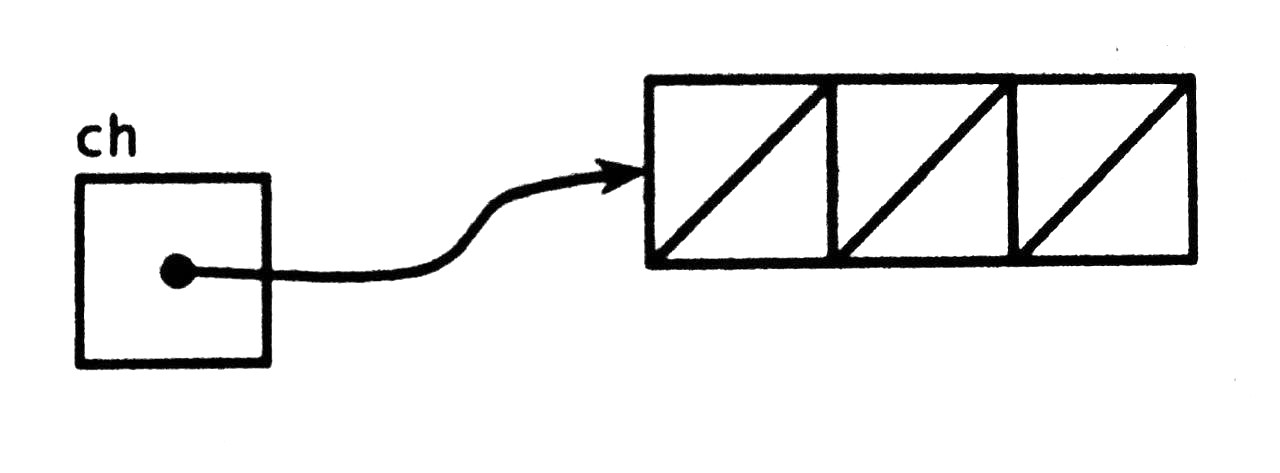
\includegraphics[scale = 0.125]{figure-8.2}
    \end{center}
    Un'operazione di send su un buffered channel inserisce un elemento in coda alla fila d'attesa , e l'operazione di receive rimove un elemento dalla testa della fila.
    Se il channel è pieno, l'operazione di send blocca la propria goroutine fino a quando non viene fatto spazio in seguito all'operazione di receive di un'altra goroutine.
    Al contrario, se il channel è vuoto, un'operazione di receive blocca la propria goroutine fino a quando un'altra goroutine non esegue un'operazione di send sullo stesso channel.
    \begin{lstlisting}[frame = single, label = {lst:lstlisting7-4-4.2}]
ch <- "A"
ch <- "B"
ch <- "C"
    \end{lstlisting}
    Dopo aver eseguito queste tre istruzioni, il channel è pieno e una quarta operazione di send verrà bloccata.
    \begin{center}
        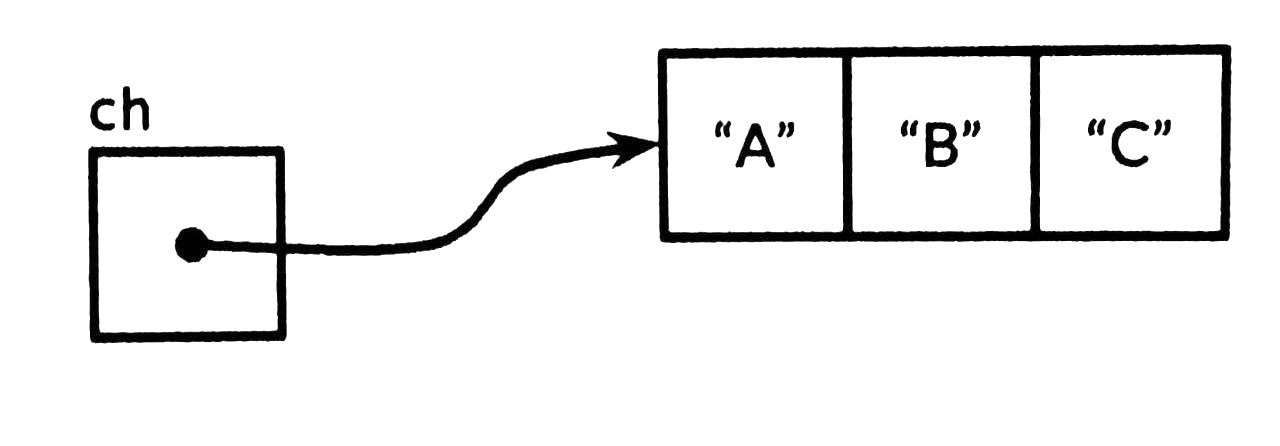
\includegraphics[scale = 0.125]{figure-8.3}
    \end{center}
    Se si riceve un valore,
    \begin{lstlisting}[frame = single, label = {lst:lstlisting7-4-4.3}]
fmt.Println(<-ch)
    \end{lstlisting}
    Output:
    \begin{lstlisting}[language = bash, frame = L, label = {lst:lstlisting7-4-4.4}]
A
    \end{lstlisting}
    il channel non sarà più nè pieno nè vuoto, quindi sia un'operazione di send che una di receive potranno procedere senza essere bloccati.
    In questo modo, il buffer del channel separa le goroutine mittenti e destinatari.
    \begin{center}
        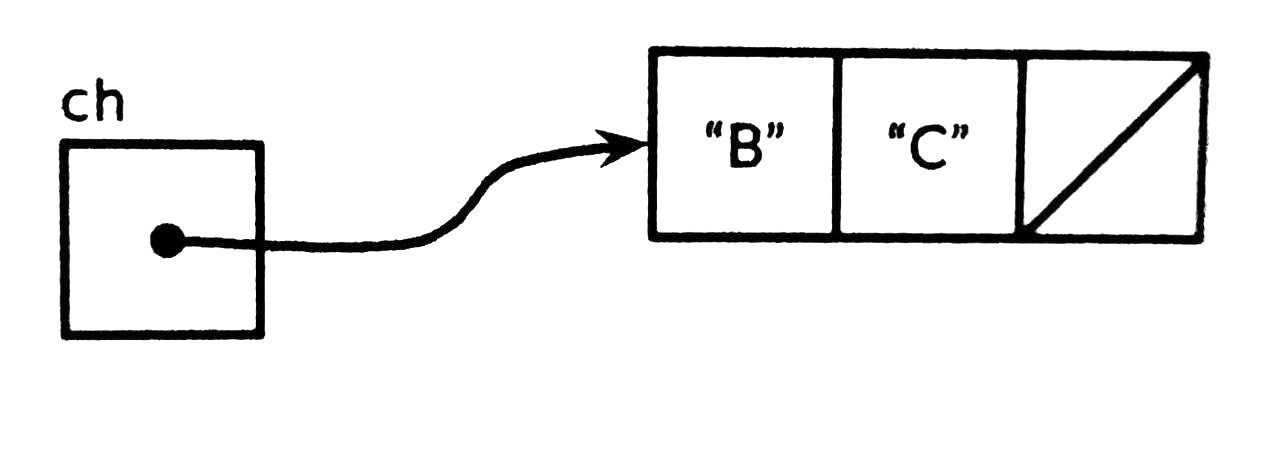
\includegraphics[scale = 0.125]{figure-8.4}
    \end{center}
    Nel caso un programma voglia conoscere la capacità del buffer del channel può richiamare la funzione \verb"cap":
    \begin{lstlisting}[frame = single, label = {lst:lstlisting7-4-4.5}]
fmt.Println(cap(ch))
    \end{lstlisting}
    Output:
    \begin{lstlisting}[language = bash, frame = L, label = {lst:lstlisting7-4-4.6}]
3
    \end{lstlisting}
    Quando applicato al channel, la funzione \verb"len" restituisce il numero di elementi al momento presenti nel buffer.
    \hfill \vspace{12pt}

    Il seguente esempio presenta un'applicazione di un buffered channel.
    Tale programma fa richieste in parallelo a tre \textit{mirror}, ovvero server equivalenti ma geograficamente distribuiti.
    Essi inviano la loro risposta su un buffered channel, quindi ricevono e restituiscono solo la prima risposta, che è la più veloce ad arrivare.
    Quindi \verb"mirrorQuery" restituisce un risultato anche prima della risposta dei due server più lenti.
    \begin{lstlisting}[frame = single, label = {lst:lstlisting7-4-4.7}]
func mirrorQuery() string {
responses := make(chan string, 3)
    go func() { responses <- request(%*``*)asia.gopl.io%*''*)) }()
    go func() { responses <- request(%*``*)europe.gopl.io%*''*)) }()
    go func() { responses <- request(%*``*)americas.gopl.io%*''*)) }()
    return <-responses // Ritorna la risposta pi%*\textit{ù}*) veloce
}

func request(hostname string) (response string) { /* ... */ }
    \end{lstlisting}
    La scelta fra un unbuffered e buffered channel e la scelta della capacity per il buffered channel possono entrambe influenzare la correttezza del programma.
    Gli unbuffered channel offrono una forte garanzia di sincronizzazione perché ogni operazione di send è sincronizzata con la corrispettiva operazione di receive;
    con i buffered channel, queste operazioni sono slegate.
    Inoltre, quando si conosce la dimensione massima del numero di valori che possono essere inviati su un channel, è utile creare un buffered channel di quella dimensione ed effettuare tutti i send ancor prima che il primo valore sia ricevuto dal destinatario.
    Un fallimento nell'allocazione di un buffer di sufficiente capacity potrebbe portare il programma ad un deadlock.
\end{document}